\documentclass[10pt]{scrreprt}
\usepackage[utf8]{inputenc}
\usepackage{amsfonts}
\usepackage{amsmath}
\usepackage{amssymb}
\usepackage{commath}
\usepackage[ngerman]{babel}
\usepackage{enumitem}
\usepackage{booktabs}
\usepackage{longtable}
\usepackage{relsize}
\usepackage{pgfplots}
\usepackage{csvsimple}
\usepackage{pgfplotstable}
\usepackage{siunitx}
\usepackage{fancyhdr}
\usepackage{color}
\usepackage{float}
\usepackage{listings}

\definecolor{mygreen}{RGB}{28,172,0} % color values Red, Green, Blue
\definecolor{mylilas}{RGB}{170,55,241}


\lstset{language=Matlab,%
%basicstyle=\color{red},
breaklines=true,%
morekeywords={matlab2tikz},
keywordstyle=\color{blue},%
morekeywords=[2]{1}, keywordstyle=[2]{\color{black}},
identifierstyle=\color{black},%
stringstyle=\color{mylilas},
commentstyle=\color{mygreen},%
showstringspaces=false,%without this there will be a symbol in the places where there is a space
%numbers=left,%
%numberstyle={\tiny \color{black}},% size of the numbers
%numbersep=9pt, % this defines how far the numbers are from the text
emph=[1]{for,end,break},emphstyle=[1]\color{red}, %some words to emphasise
%emph=[2]{word1,word2}, emphstyle=[2]{style},
}

\setlength\parindent{0pt}

\setcounter{chapter}{5}
\setcounter{secnumdepth}{3}
\setcounter{figure}{12}


\pagestyle{fancy}
\fancyhf{}
\lhead{GPET Versuch 7}
\rhead{Tim Luchterhand, Paul Nykiel}
\cfoot{\thepage}

\author{Tim Luchterhand, Paul Nykiel \protect\\ tim.luchterhand@uni-ulm.de, paul.nykiel@uni-ulm.de}
\title{GPET Versuch 7 --- Operation John Ragazzini}
\subtitle{Gruppe: Dienstag14}

\begin{document}
    \maketitle
    \section{Untersuchung von Spannungsfolgern}
    \begin{center}
        \begin{figure}[H]
            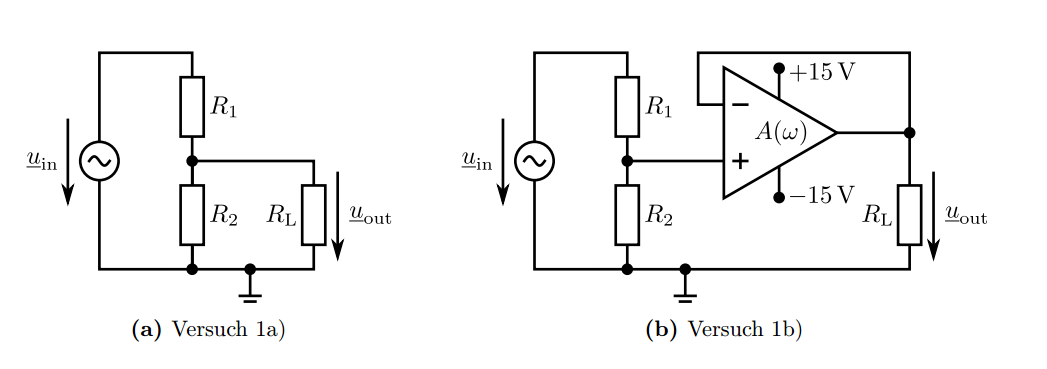
\includegraphics[width=\textwidth]{abb14.png}
            \caption{Spannungsfolger.}
            \label{fig:abb14}
        \end{figure}
    \end{center}
    \subsection{Belasteter Spannungsteiler}
    Bauen Sie zunächst die Schaltung nach Abbildung~\ref{fig:abb14}a auf. Die Eingangsspannung soll
    $u_{in} = 5\si{\volt}$ DC und die Widerstände $R_1 = R_2 = 1\si{k\ohm}$ sowie $R_L = 220\si{\ohm}$ betragen.
    Messen Sie mit dem Multimeter die über den Lastwiderstand abfallende Spannung $u_{out}$.

    \vspace{0.5cm}

    Erklären Sie das Ergebnis?

    \paragraph{Protokol}

    Durch den Lastwiderstand $R_L$ wird der Spannungsteiler belastet und verhält
    sich anders, als unbeastet.
    Die Ausgansspannung lässt sich dann berechnen durch:
    \begin{eqnarray*}
        R_{2 \vert L} &=& \frac{R_2 R_l}{R_2 + R_L} \\
        u_{out} &=& u_{in} \frac{R_{2 \vert L}}{R_{2 \vert L}+R_1} = 0.764\si{\volt}
    \end{eqnarray*}

    Dieser Wert konnte durch Messung bestätigt werden:
    \begin{equation*}
        u_{out, mess} = 0.755\si{\volt}
    \end{equation*}

    \subsection{Belasteter Spannungsfolger}
    Erweitern Sie nun den Aufbau um einen Spannungsfolger wie in Abbildung~\ref{fig:abb14}b. Der OP
    benötigt eine Betriebsspannung von $\pm 15\si{\volt}$.

    Messen Sie wiederum die Spannung über dem Lastwiderstand mit dem Multimeter.

    \vspace{0.5cm}

    Erklären Sie das Ergebnis und geben Sie ein Beispiel an, wozu diese Schaltung Verwendet
    werden könnte?

    \paragraph{Protokoll}
    Der OP belastet den Spannungsteiler durch seine hohen Eingangswiderstände
    nur geringfügig, weshalb sich die Schaltung auch mit Lastwiderstand wie ein
    unbelasteter Spannungsteiler verhält. Dementsprechend gilt für die Ausgangsspannung:
    \begin{equation*}
        u_{out} = \frac{R_2}{R_1+R_2} u_{in} = \frac{1}{2}\cdot 5\si{\volt} = 2.5\si{\volt}
    \end{equation*}

    Auch hier bestätigt die Messung die Theorie:
    \begin{equation*}
        u_{out} = 2.447\si{\volt}
    \end{equation*}

    \subparagraph{Bemerkung}
    Der OP konnte im eingebauten Zustand nur bis auf ein Offset von $1.0\si{m\volt}$
    abgeglichen werden.

    \vspace{0.5cm}

    Mit diesem Aufbau kann also von belieigen Schaltungen Leistung abgegriffen
    werden, ohne dass die Schaltung selbst beeinflusst wird. Ein Einsatzgebiet
    sind Spannungsmessinstrumente, die die untersuchte Schaltung schließlich
    nicht beeinflussen sollen.

    \section{Charakterisierung der Verstärkung}
    \begin{center}
        \begin{figure}[H]
            
\includegraphics[width=\textwidth]{abb8.png}
            \caption{Invertierender Verstärker}
            \label{fig:abb8}
        \end{figure}
    \end{center}
    Bauen Sie eine Schaltung nach Abbildung~\ref{fig:abb8} mit $R_1 = 1\si{k\ohm}$ und einer Betriebsverstärkung
    von $A_B = 10$ auf. Schalten Sie für diesen Versuch zusätzlich zwischen dem positiven
    Eingang des OPs und der Masse einen $220\si{k\ohm}$ Widerstand.

    \subparagraph{Bemerkung}
    Um die angegebene Verstärkung zu realisieren wurde ein $10\si{k\ohm}$ Widerstand
    als $R_1$ verwendet.




    \subsection{Abhängigkeit von der Eingangsamplitude}
    Verwenden Sie als Eingangsspannung ein sinusförmiges Signal mit $f = 1\si{k\hertz}$ und
    Amplituden gemäß der unten stehenden Tabelle. Tragen Sie die gemessene Ausgangsamplitude
    in die Tabelle ein und berechnen Sie anschließend die Verstärkung.

    Erklären Sie das Ergebnis insbesondere ab $3\si{\volt}$ Eingangsspannung? Wie könnte man das
    Problem lösen? Beschreiben Sie die Phasenbeziehung zwischen Ein- und Ausgangssignal.
    Führen Sie nun mithilfe der Matlab-GUI dieselbe Messung noch einmal durch und
    übernehmen Sie das Diagramm in ihre Auswertung.

    \paragraph{Protokoll}
    $ $

    \begin{table}[H]
        \begin{center}
            \pgfplotstabletypeset[
            multicolumn names, % allows to have multicolumn names
            col sep=space, % the seperator in our .csv file
            display columns/0/.style={
            column name=$u_{in}$, % name of first column
            column type={S},string type},  % use siunitx for formatting
            display columns/1/.style={
            column name=$u_{out}$,
            column type={S},string type},
            display columns/2/.style={
            column name={$A_B$ = $u_{out} / u_{in}$},
            column type={S},string type},
            display columns/3/.style={
            column name=$20dB\log_{10} (A_B)$,
            column type={S},string type},
            every head row/.style={
            before row={\toprule}, % have a rule at top
            after row={
            $\si{\volt}$ & $\si{\volt}$ &  & $\text{dB}$ \\
            \midrule} % rule under units
            },
            every last row/.style={after row=\bottomrule},
            ]{taba.csv}
        \end{center}
    \end{table}

    \begin{center}
        \begin{figure}[H]
            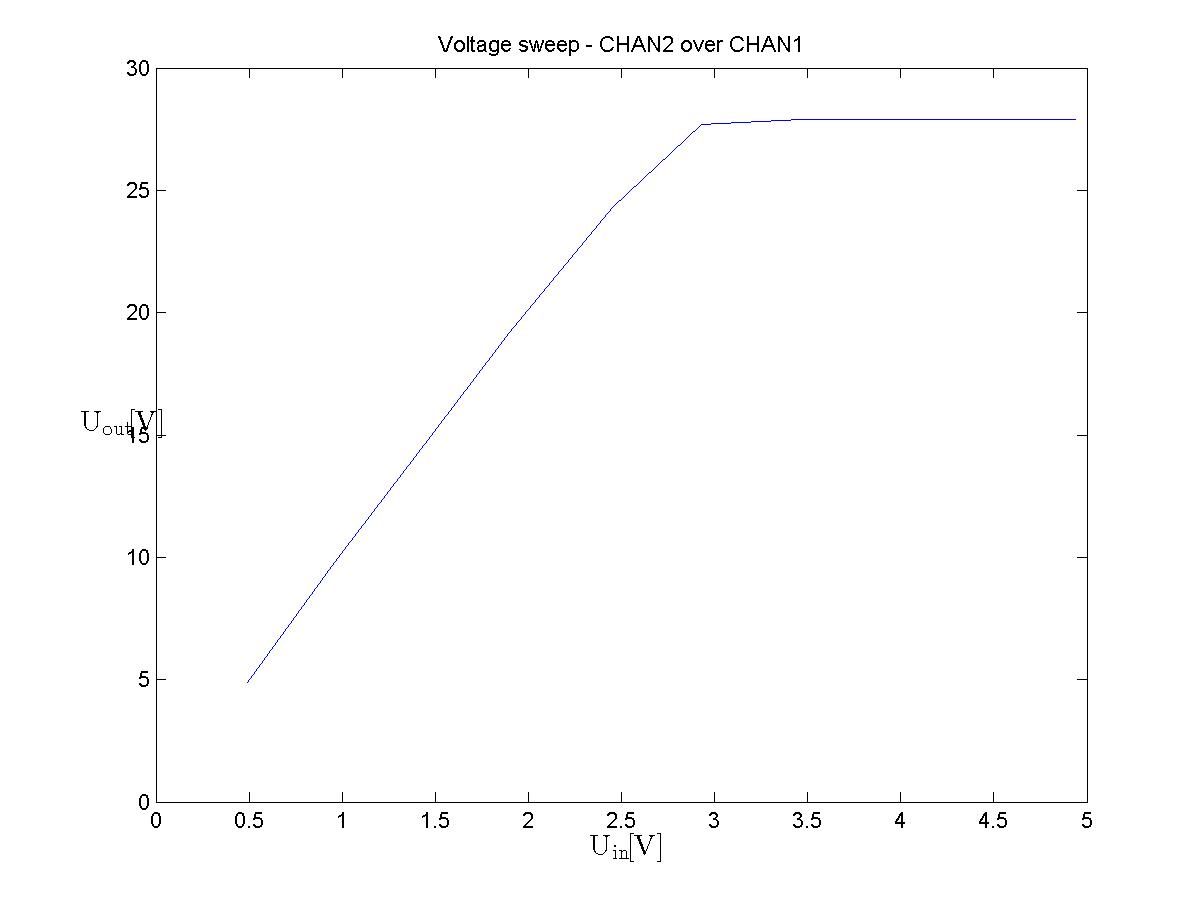
\includegraphics[width=\textwidth]{VS521_voltagesweep.jpg}
            \caption{Voltage sweep des invertierten Verstärkers}
        \end{figure}
        \begin{figure}[H]
            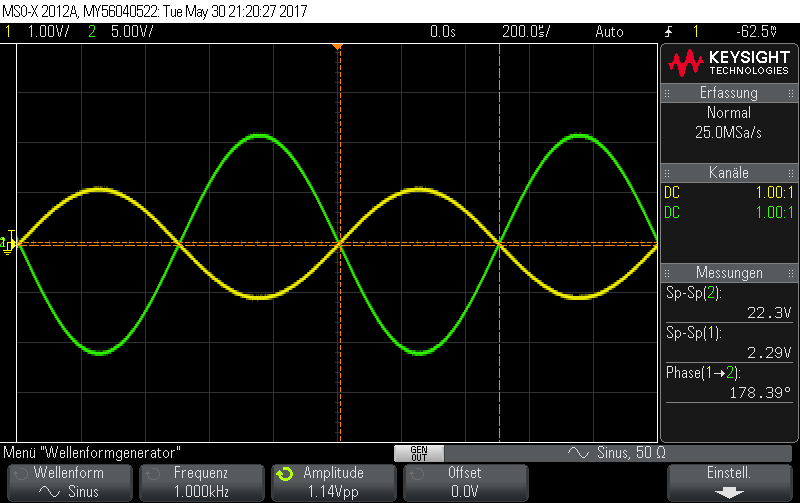
\includegraphics[width=\textwidth]{scope_5.png}
            \caption{Phasenbeziehung zwischen Ein- und Ausgangsspannung}
            \label{fig:Phasenbez}
        \end{figure}
    \end{center}

    \subparagraph{Erklärung zur Verstärkung}
    Bei einer Eingangsspannung mit Spitze-Spitze-Spannung zwischen $0.5\si{\volt}$
    und $3\si{\volt}$ Liegt die Ausgangsspannung des OPs unter der Versorgungsspannung.
    Der OP arbeitet also wie erwartet und verstärkt das Eingangssignal um den Faktor 10.
    Die Ausgangsspannung ist also wie zu erkennen 10 mal höher, als die Eingangsspannung.

    Ab einer Spitze-Spitze-Spannung von über $3\si{\volt}$ müsste der OP eine
    Ausgansǵsspanung von über $15\si{\volt}$ liefern, was nicht möglich ist, da
    dieser Wert über der bereitgestellten Versorgungsspannung liegt. Der OP stellt
    also immer die höchstmögliche Ausgansspannung von $15\si{\volt}$PP zur Verfügung.

    \subparagraph{Erklärung zur Phase}
    Wie in Grafik~\ref{fig:Phasenbez} zu erkennen, sind Ein- und Ausgangsspannung
    um ca. $180^\circ$ phasenverschoben. Die verwendete Schaltung ist ein invertierender
    Verstärker. D.h. Ein- und Ausgangsspannung haben ein unterschiedliches Vorzeichen,
    was genau einer Phasenverschiebung von $180^\circ$ entspricht.


    \subsection{Abhängigkeit von der Eingangsfrequenz}
    Stellen sie nun bei einer Eingangsspannung von $u_{in} = 2\si{\volt}_{pp}$ verschiedene Frequenzen
    gemäß unten stehender Tabelle ein. Tragen Sie wiederum die gemessenen Amplituden der
    Ausgangsspannung in die Tabelle ein und berechnen Sie anschließend die Verstärkung.

    Bei welcher Frequenz ist die Ausgangsspannung um 3 dB abgesunken und wie nennt man
    diese Frequenz?
    Führen Sie mit Matlab einen automatischen Frequenzsweep durch und fügen Sie das
    resultierende Diagramm in die Auswertung ein.

    \paragraph{Protokoll}
    $ $

    \begin{table}[H]
        \begin{center}
            \pgfplotstabletypeset[
            multicolumn names, % allows to have multicolumn names
            col sep=space, % the seperator in our .csv file
            display columns/0/.style={
            column name=$f$,
            column type={S[round-mode=figures, round-precision=1, scientific-notation=engineering, table-format=1e1]},string type},
            display columns/1/.style={
            column name=$u_{in}$, % name of first column
            column type={S},string type},  % use siunitx for formatting
            display columns/2/.style={
            column name=$u_{out}$,
            column type={S},string type},
            display columns/3/.style={
            column name={$A_B$ = $u_{out} / u_{in}$},
            column type={S},string type},
            display columns/4/.style={
            column name=$20dB\log_{10} (A_B)$,
            column type={S},string type},
            every head row/.style={
            before row={\toprule}, % have a rule at top
            after row={
            $\si{\hertz}$ & $\si{\volt}$ & $\si{\volt}$ &  & $\text{dB}$ \\
            \midrule} % rule under units
            },
            every last row/.style={after row=\bottomrule},
            ]{tabb.csv}
        \end{center}
    \end{table}
    \begin{center}
        \begin{figure}[H]
            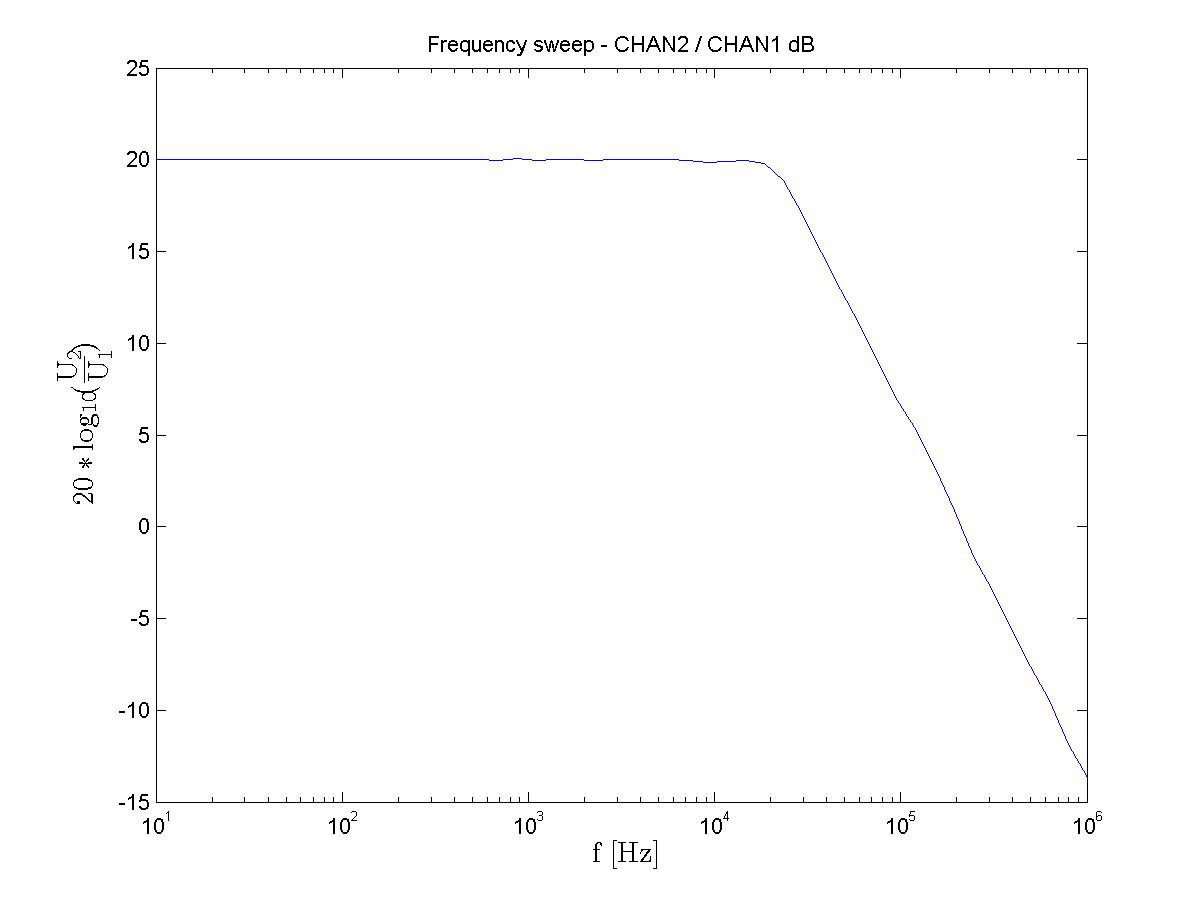
\includegraphics[width=\textwidth]{FS522_frequencysweep_ylogxlog.jpg}
            \caption{Frequenzsweep mit Matlab}
            \label{fig:Matlab52b}
        \end{figure}
    \end{center}

    Wie in Grafik~\ref{fig:Matlab52b} zu erkennen, bleibt die Verstärkung des OPs
    bis zur Grenzfrequenz $f_g \approx 50\si{k\hertz}$ konstant bei 20db und fällt
    dann mit 20dB pro Dekade ab.

    Bei einer Frequenz von ca. $50\si{k\hertz}$ ist die Ausgangsspannung um
    3dB gesunken. Diese Frequenz nennt man Grenzfrequenz.

    \section{Auswertung einer Addierer-Schaltung}
    \begin{center}
        \begin{figure}[H]
            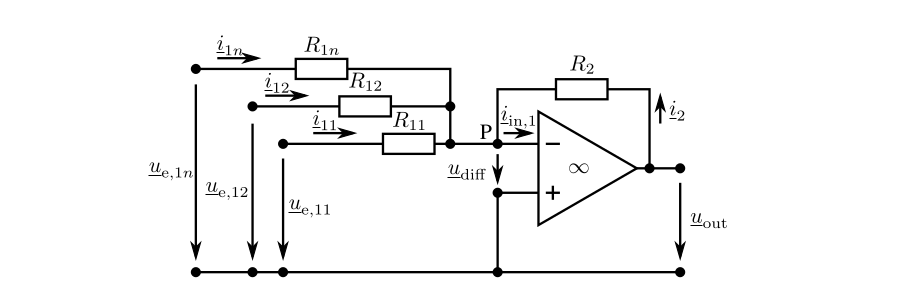
\includegraphics[width=\textwidth]{abb10.png}
            \caption{Addier-Schaltung}
            \label{fig:abb10}
        \end{figure}
    \end{center}
    Bauen Sie eine Schaltung gemäß Abbildung~\ref{fig:abb10} mit lediglich zwei Eingängen auf.
    Verwenden Sie dazu $R_{11} = 300\si{\ohm}$, $R_{12} = 200\si{\ohm}$ und $R_2 = 500\si{\ohm}$. Schalten Sie wiederum zusätzlich
    zwischen dem positiven Eingang des OPs und der Masse einen $220\si{k\ohm}$ Widerstand.
    Legen Sie nun eine Wechselspannung von $u_{e,1} = 2.5\si{\volt}_{pp}$ und einer Frequenz von $1\si{k\hertz}$
    an. Dazu soll eine Gleichspannung von $u_{e,2} = 2.5\si{\volt}$ addiert werden. Berechnen Sie die
    jeweiligen Verstärkungsfaktoren der einzelnen Eingangspfade. Messen Sie nun die
    Ausgangsspannung und vergleichen Sie die berechneten Ergebnisse mit den praktisch
    gemessenen.

    \paragraph{Protkoll}
    \begin{center}
        \begin{figure}[H]
            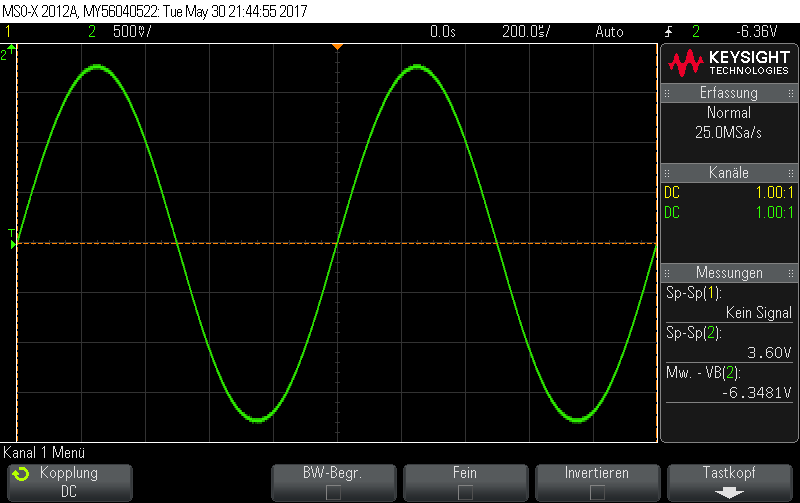
\includegraphics[width=\textwidth]{scope_6.png}
            \caption{Gleichanteil des Summensignals}
        \end{figure}
    \end{center}

    Die Verstärkungsfaktoren der einzelnen Eingänge lassen sich wie folgt berechen:
    \begin{eqnarray*}
        A_1 &=& -\frac{R_2}{R_{11}} = -\frac{5}{3}\\
        A_2 &=& -\frac{R_2}{R_{12}} = -\frac{5}{2}\\
    \end{eqnarray*}

    Die Ausgangsspannung lässt sich dann folgendermaßen berechnen:

    \begin{eqnarray*}
        &u_{out}& = A_1 u_1 + A_2 u_2 = -\frac{5}{3} u_1 -\frac{5}{2} u_2 =
        (-\frac{25}{12}\sin(\omega t) - \frac{25}{4})\si{\volt}\\
        \Rightarrow &u_{out,Gleichanteil}& = -\frac{25}{4}\si{\volt} = -6.25\si{\volt}
    \end{eqnarray*}

    Die Messung bestätigt die Theorie:
    \begin{equation*}
        u_{out,Gleichanteil} = -6.35\si{\volt}
    \end{equation*}

    \section{Auswertung einer Integrator-Schaltungen}
    \begin{center}
        \begin{figure}[H]
            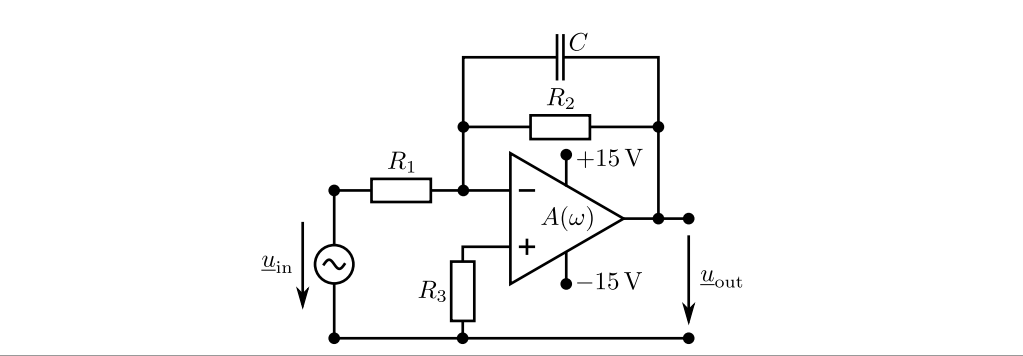
\includegraphics[width=\textwidth]{abb15.png}
            \caption{Integrator-Schaltung.}
            \label{fig:abb15}
        \end{figure}
    \end{center}
    Bauen Sie die Schaltung aus Abbildung~\ref{fig:abb15} auf.
    Verwenden Sie dazu $u_{in} = 2\si{\volt}_{pp}$, $R_1 = R_2 = 1\si{k\ohm}$, $R_3 = 220\si{k\ohm}$ und $C = 1.5\si{n\farad}$.
    Stellen Sie verschiedene Frequenzen für die Eingangsspannung ein und beobachten Sie
    mit dem Oszilloskop was passiert.
    \begin{itemize}
        \item Ab wie viel Hz funktioniert die Integration? (ab wann sieht die Ausgangsspannung
            wie erwartet aus?)
        \item Welche Phasenverschiebung liegt zwischen Eingangs- und Ausgangsspannung und
            warum?
        \item Was passiert wenn man statt dem Sinus einen Dreieck oder ein Rechteck auf den
            Eingang des Integrators gibt und warum?
    \end{itemize}
    Nehmen Sie mit Matlab den Frequenzgang von $100\si{\hertz} - 1\si{M\hertz}$ auf und fügen Sie das
    Diagramm in die Auswertung ein.
    Machen Sie mit dem Oszilloskop einen Screenshot von der Integration einer Dreiecks- und
    einer Rechtecksspannung und diskutieren Sie Ihre Ergebnisse.

    \paragraph{Protokoll}
    \begin{center}
        \begin{figure}[H]
            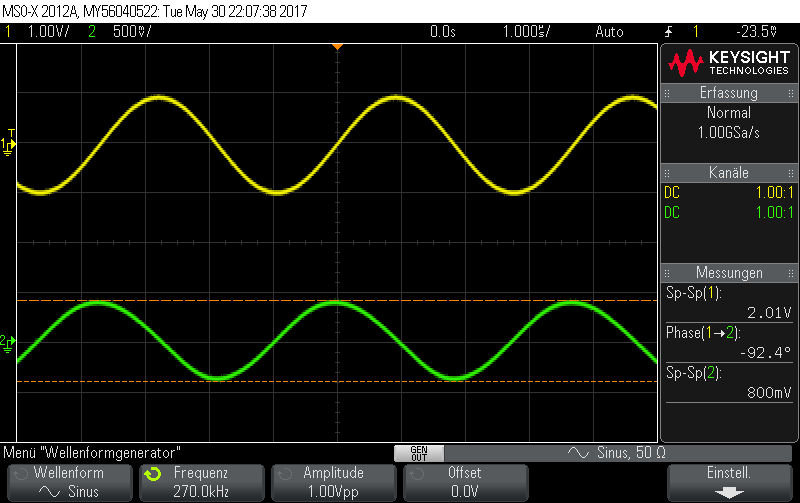
\includegraphics[width=\textwidth]{scope_7.png}
            \caption{Integration eines Sinussignals}
        \end{figure}
    \end{center}

    Bei ca.~$270\si{k\hertz}$ funktioniert der Integrator ordnungsgemäß, da dann
    Ein- und Ausgangsspannung um $90^\circ$ phasenverschoben sind.
    Diese Phasenverschiebung entsteht durch die Integration des Sinus, der zu einem
    Kosinus wird.

    \begin{center}
        \begin{figure}[H]
            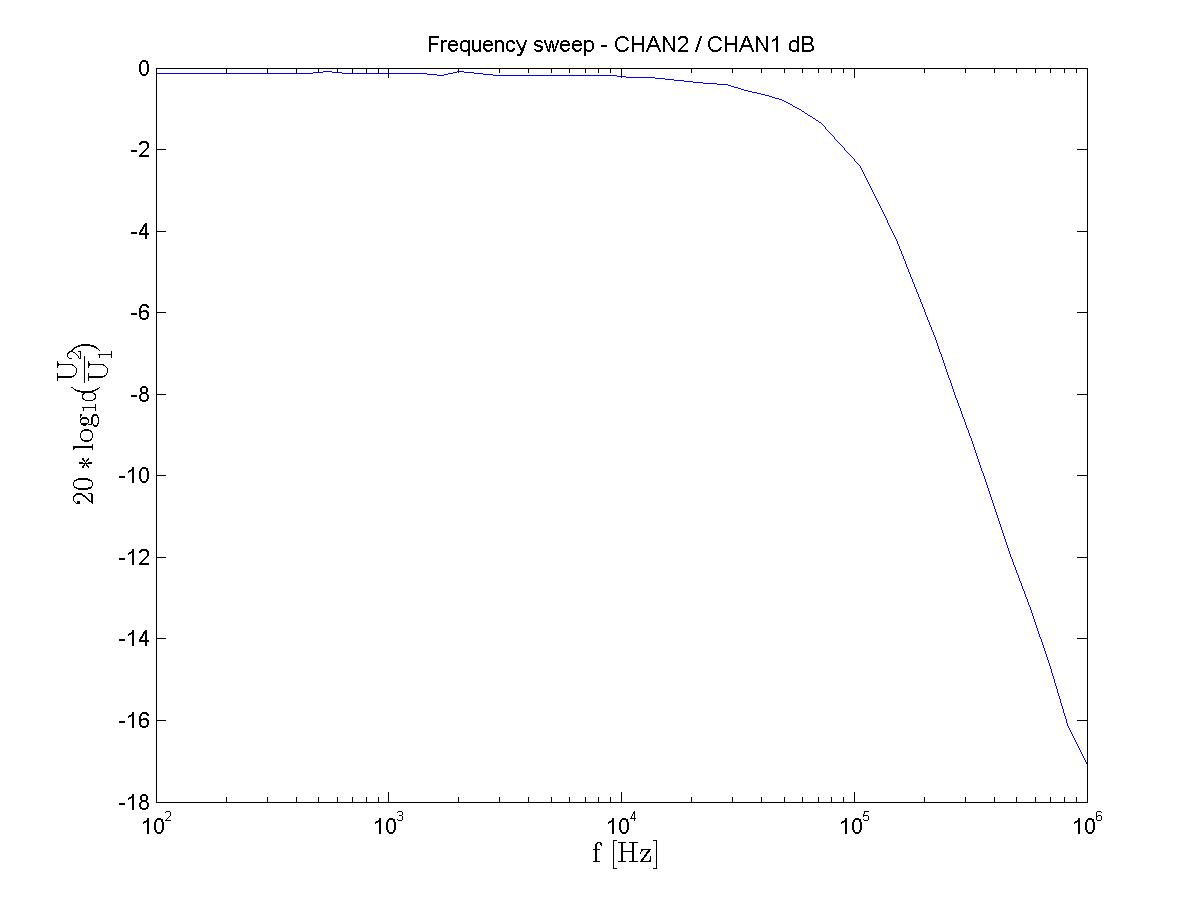
\includegraphics[width=0.9\textwidth]{FS54_frequencysweep_ylogxlog.jpg}
            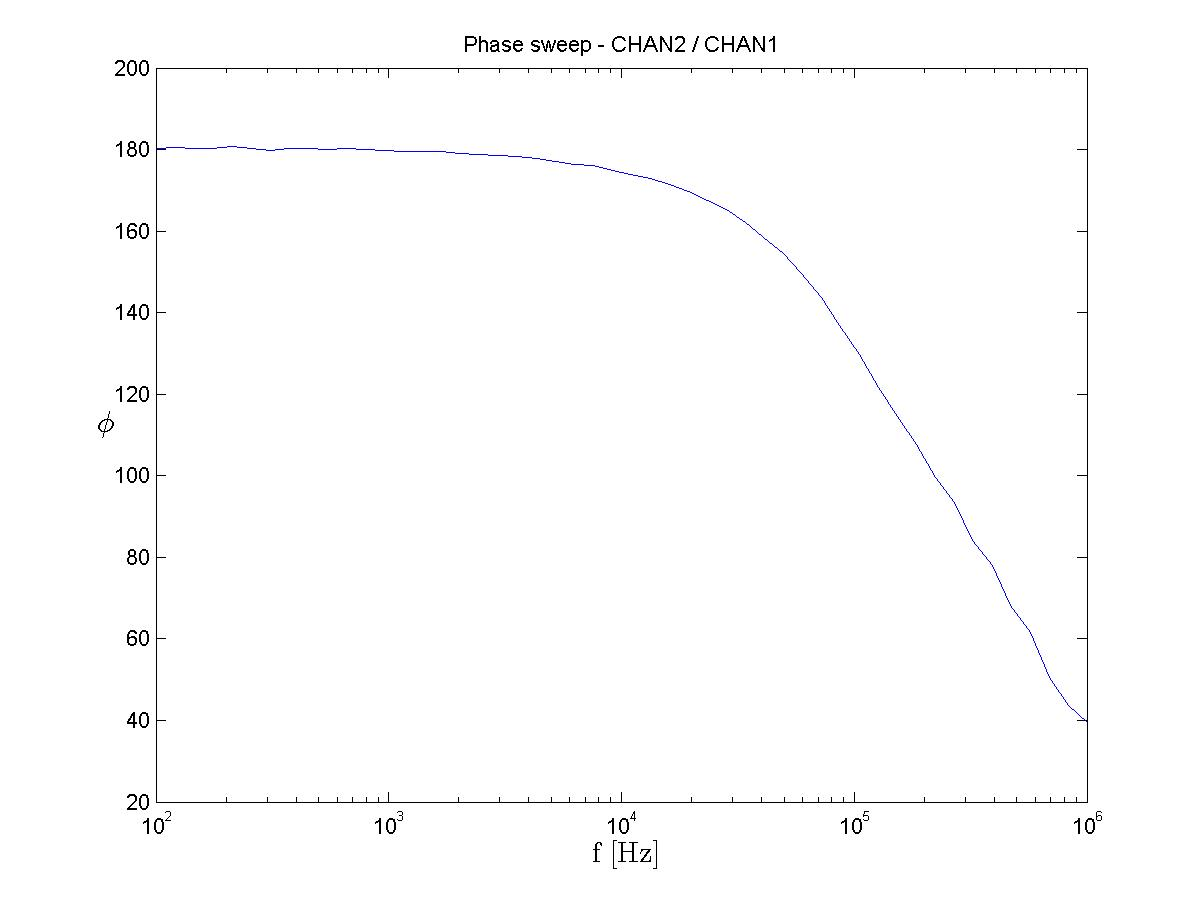
\includegraphics[width=0.9\textwidth]{PS54_phasesweep_xlog.jpg}
            \label{fig:Bod}
            \caption{Bode-Diagramm des Integrators}
        \end{figure}
    \end{center}


    \begin{center}
        \begin{figure}[H]
            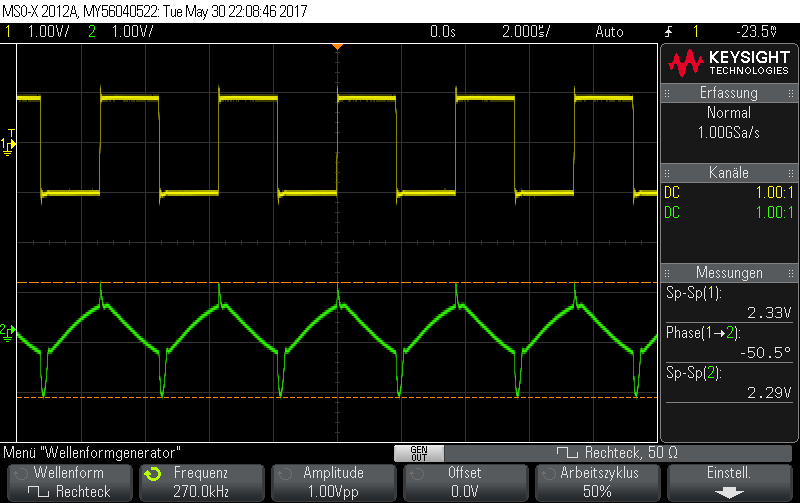
\includegraphics[width=\textwidth]{scope_8.png}
            \caption{Integration eines Rechtecksignals}
        \end{figure}
    \end{center}
    \begin{center}
        \begin{figure}[H]
            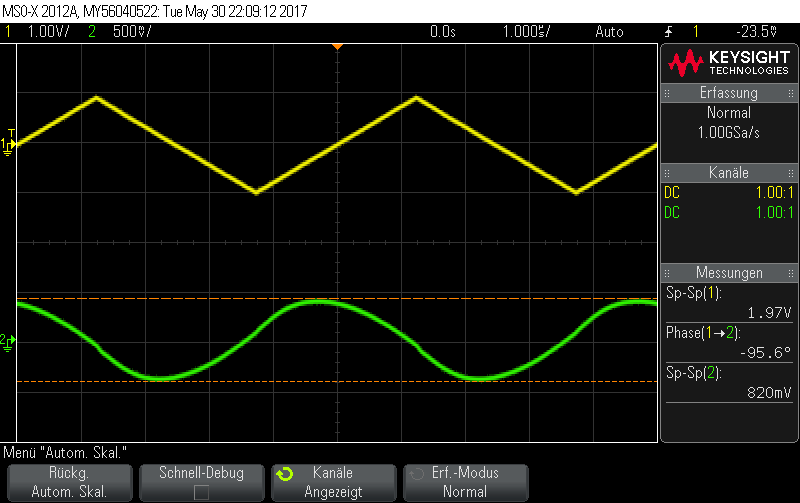
\includegraphics[width=\textwidth]{scope_9.png}
            \caption{Integration eines Sägezahnsignals}
        \end{figure}
    \end{center}

    Durch den Integrator ändert sich ein am Eingang angelegtes Rechtscksignal
    zu einem dreiecksförmigen Signal.

    Ein Sägezahnsignal wird durch Integrieren zu einem sinusartigen Signal.

    \vspace{1cm}

    Modifizieren Sie im Weiteren obige Schaltung folgendermaßen:
    $u_{in} = 2\si{\volt}_{pp}$, $R_1 = R_2 = 10\si{k\ohm}$, $R_3 = 0\si{\ohm}$ und $C = 1.5\si{n\farad}$.
    Nehmen Sie mit Matlab den Frequenzgang von $10\si{\hertz} - 100\si{k\hertz}$ auf und fügen Sie das
    Diagramm in die Auswertung ein. Wozu kann diese Schaltung noch verwendet werden?
    Erklären Sie die Funktion der Schaltung.
    \begin{center}
        \begin{figure}[H]
            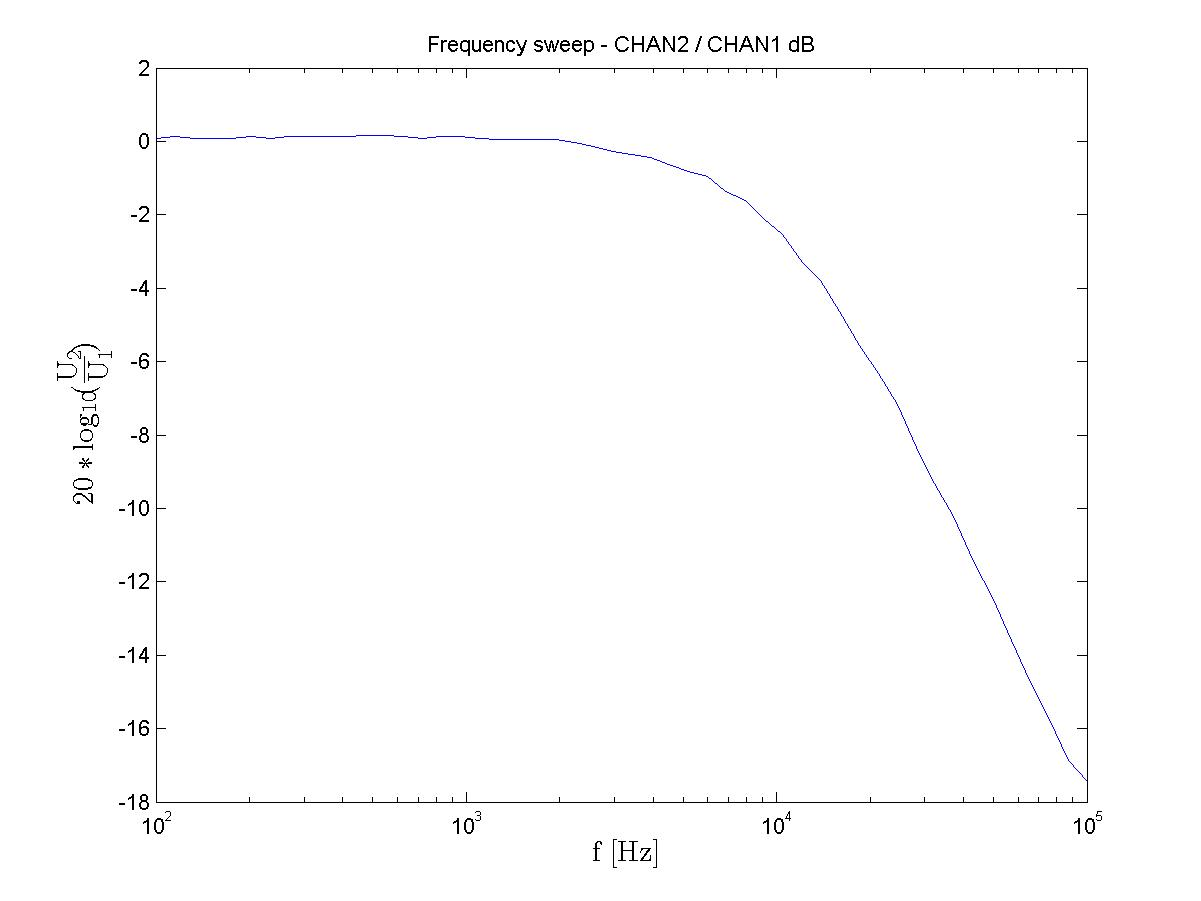
\includegraphics[width=0.9\textwidth]{FS542_frequencysweep_ylogxlog.jpg}
            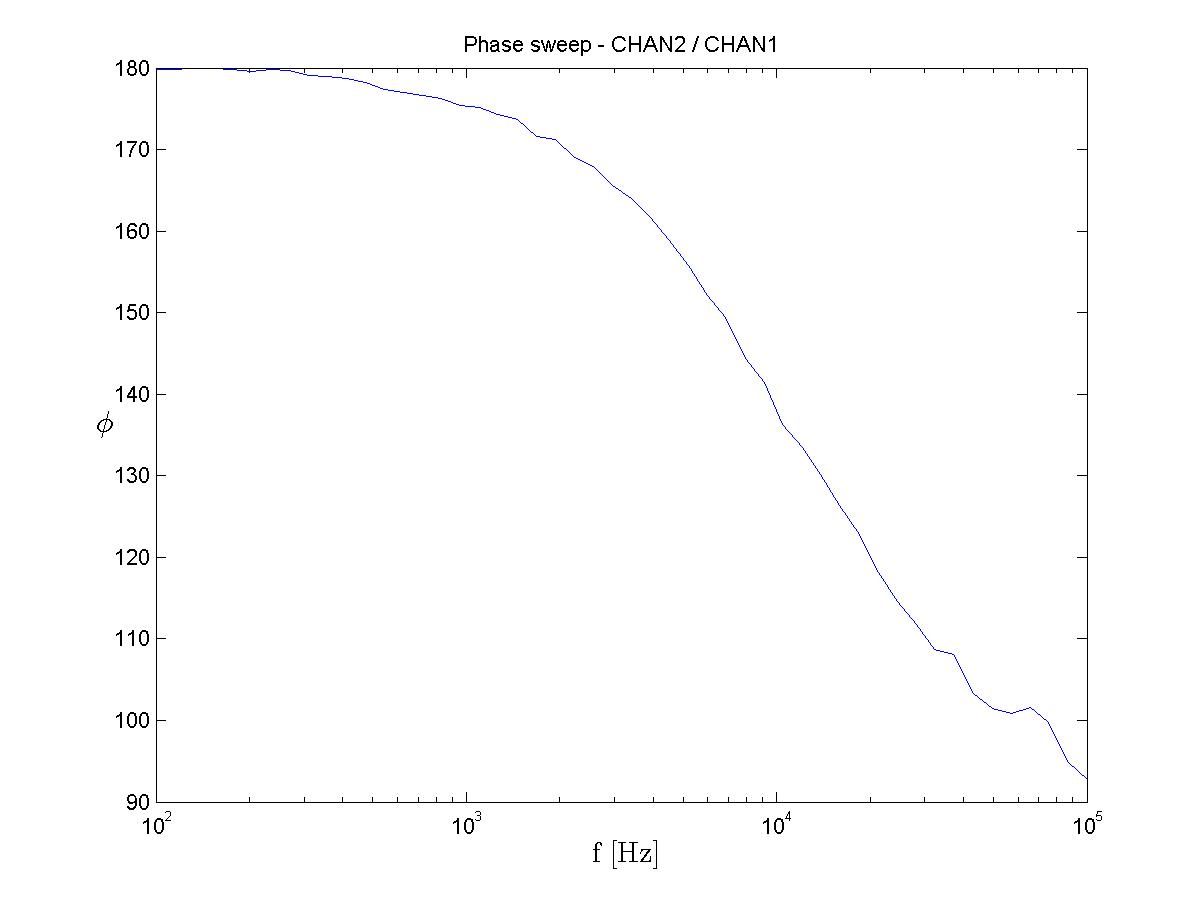
\includegraphics[width=0.9\textwidth]{PS542_phasesweep_xlog.jpg}
            \caption{Bode-Diagramm des modifizierten Integrators}
            \label{fig:BodMod}
        \end{figure}
    \end{center}
    Vergleicht man Grafik~\ref{fig:Bod} und Grafik~\ref{fig:BodMod}, so  erkennt
    man, dass der modifizierte Integrator eine deutlich niedrigere Grenzfrequenz
    (bei ca.~$10\si{k\hertz}$) besitzt.
\end{document}
